\documentclass{article}

\usepackage[ansinew]{inputenc} %Bærbar ÆØÅ?

\usepackage{amsmath}
\usepackage{minted}
\usepackage{graphicx} % Allows figures
\usepackage{tabularx}
\usepackage{etoolbox} %for configuration of sloppy

%Section style
\usepackage{xcolor}

\definecolor{secnum}{RGB}{102,102,102}

\makeatletter
    \def\@seccntformat#1{\llap{\color{secnum}\csname the#1\endcsname\hskip 16pt}}
\makeatother
%end section style

{\sloppy}{\hbadness 10000\relax}{}{} %adds hbadness to sloppy
\setlength{\paperheight}{297mm} %Sets the page to an A4
\setlength{\paperwidth}{210mm}        %Sets the page to an A4

\begin{document}

\begin{titlepage}
\begin{center}
\textsc{Introduction to Graphics}\\[0.5cm]
\textsc{Assignment 2: Geometriske Transformationer}\\[0.5cm]
\vspace{2 cm}
\begin{tabular}{ll}
Student: & Kasper Passov\\
\end{tabular}
\end{center}
\vspace{5 cm}
\newpage
\end{titlepage}

\section{Problem description}

% \subsection{Problem description (religious)}
% On the first day, The Helix created the triangle. The great Helix
% placed the triangle in a box of darkness and democrazy. The great one
% saw this would not do, and therefore functions was needed to absolve
% the triangle from it's way of heresy and bring it into anarchy.
% This would need the great function trinity. Translocation, Scalation
% and Rotation. With these holy three, and the unholy one shear, the
% triangle would be able to free itself from the tyrany of democrazy
% and into the great ones way of anarchy.

\subsection{Problem description}
We want functions that enable us to transform triangles, so that
any triangle can be transformed into any other triangle.


\subsection{Scale}

Scaling enables us to grow and shrink the triangle, whithout 
modifying the sides ratio. 
This is done using matrix transformations with the vector equation\\
$
\begin{bmatrix}
xnew \\
ynew
\end{bmatrix} = 
\begin{bmatrix} s_{x} & 0 \\ 0 & s_{y} \end{bmatrix} 
\begin{bmatrix} xorg \\ yorg \end{bmatrix}
$\\
This is just multiplying the scale factor with the position.

\subsection{Rotate}

Rotation is found by the vector equation\\
$
\begin{bmatrix} xnew \\ ynew \end{bmatrix} =
\begin{bmatrix} cos_{\Theta} & -sin_{\Theta} \\ sin{\Theta} & cos_{\Theta} \end{bmatrix} 
\begin{bmatrix} xorg \\ yorg \end{bmatrix}
$\\
\subsection{Translocation}

\subsubsection{Homogen coordinates}
The problem with the simple implementation of translocation is
it uses addition, where the other transformations uses multiplication.
This mean we would have to create speciel cases to handle translocation,
which is not an attractive attribute. 
For this we use Homogeneous Coordinates which is has one ekstra dimension. 

\subsubsection{Translocate transformation}
Translocation under Homogen coordinates is done by\\
$\begin{bmatrix} wxnew \\ wynew \\ w \end{bmatrix} =
\begin{bmatrix} 1 & 0 & d_{x} \\ sin{\Theta} & cos_{\Theta} \end{bmatrix} 
\begin{bmatrix} xorg \\ yorg \end{bmatrix}$

\section{Implementation}
I used the zipped skeleton \emph{skeletet til geometriske transformationer},
that i made work with a magic makefile i found on the forum.\\
In the skeleton i created a function that observes keystrokes, and
runs glm transformations based on the keystroke. This means i am
using the skeletons glm::(scale, rotate and translate) functions
instead of implementing my own.

\subsection{Comments on implementation}

I used the glm::(transformations) to do the transformations needed.
Furthermore i created an observer that checks for keystrokes. On each of these
keystrokes it does one of the following actions:
\begin{itemize}
    \item{a:} Scales the triangle up 
    \item{q:} Scales the triangle down
    \item{s:} Rotates the triangle clockwise
    \item{w:} Rotates the triangle counterclockwise
    \item{j:} Translocate the triangle left
    \item{l:} Translocate the triangle right 
    \item{i:} Translocate the triangle up
    \item{k:} Translocate the triangle down 
\end{itemize}
using the fitting glm::(transformation).

\subsection{The implementation}
\begin{minted}{cpp}
static void processNormalKey(unsigned char key, int x, int y) {
    glClear(GL_COLOR_BUFFER_BIT);

	triangleShaderProgram.useProgram();

	glUniformMatrix4fv(glGetUniformLocation(triangleShaderProgram.getProgram(), "uModelMatrix"), 1, GL_FALSE, glm::value_ptr(modelMatrix));

    modelMatrix = callWithKey(key);

	triangle.draw();
    glutSwapBuffers();
}

static void renderSceneCB() {
    glClear(GL_COLOR_BUFFER_BIT);

	triangleShaderProgram.useProgram();

	glUniformMatrix4fv(glGetUniformLocation(triangleShaderProgram.getProgram(), "uModelMatrix"), 1, GL_FALSE, glm::value_ptr(modelMatrix));

	glUniform1f(glGetUniformLocation(triangleShaderProgram.getProgram(), "uScale"), 0.25f);
	glUniform3f(glGetUniformLocation(triangleShaderProgram.getProgram(), "uColour"), 1.0f, 1.0f, 0.4f);
	triangle.draw();

    glutSwapBuffers();
}

glm::mat4 callWithKey(unsigned char key) {
    switch(key) {
        case 65: case 97: //a scale down 
            return glm::scale(modelMatrix, glm::vec3(0.9f,0.9f,0.0f));
            break;
        case 83: case 115: //s roate neg 
            return glm::rotate(modelMatrix, -5.0f, glm::vec3(0.2f,0.2f,0.2f));
            break;
        case 81: case 113: //q scale up
            return glm::scale(modelMatrix, glm::vec3(1.1f,1.1f,0.0f));
            break;
        case 87: case 119: //w roate pos
            return glm::rotate(modelMatrix,  5.0f, glm::vec3(0.2f,0.2f,0.2f));
            break;
        case 106:  //left j
            return glm::translate(modelMatrix, glm::vec3(-0.01f,0.0f,0.0f));
            break;
        case 105:  //up i
            return glm::translate(modelMatrix, glm::vec3(0.0f,0.01f,0.0f));
            break;
        case 108:  //right l
            return glm::translate(modelMatrix, glm::vec3(0.01f,0.0f,0.0f));
            break;
        case 107:  //down k
            return glm::translate(modelMatrix, glm::vec3(0.0f,-0.01f,0.0f));
            break;
        case 27 : //esc
            exit(0);
    }
    return modelMatrix;
\end{minted}
\newpage
\section{Testing}
I used the given framework implementing the keys describer above. 
Figure 1 (left), is the triangle before any transformations, Figure 2 (right)
is after some scaletion, translocation and rotation.\\

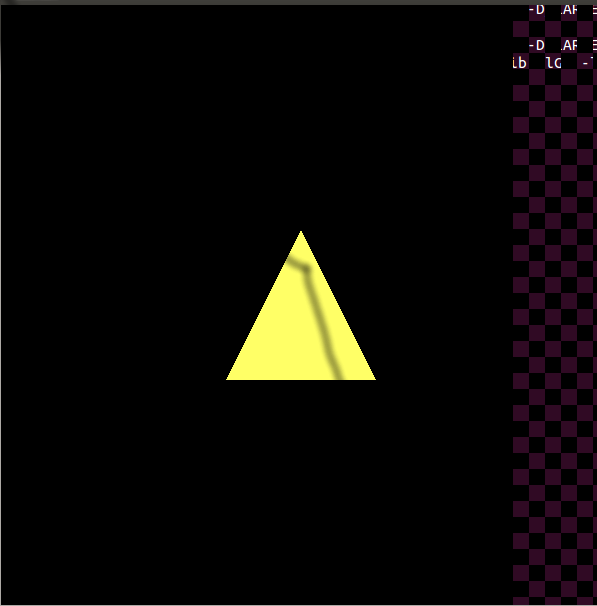
\includegraphics[scale=0.2]{penis1.png}
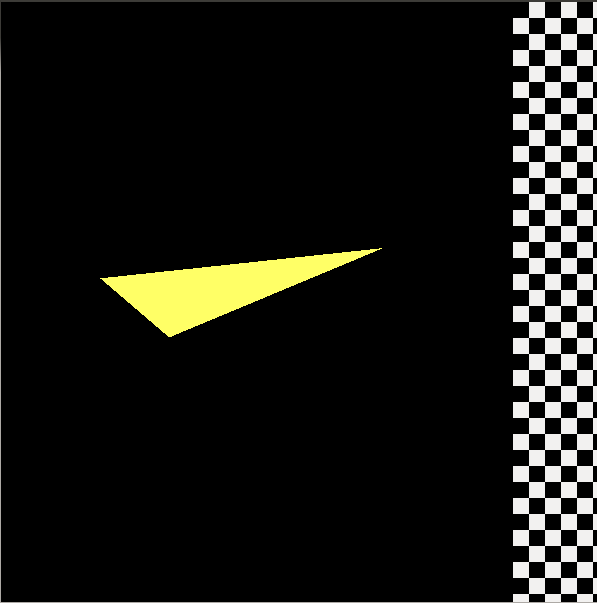
\includegraphics[scale=0.2]{penis2.png}\\
The code has been included in a zipfile and can be run and tried with the commands
defined in section 3.1. The program can be exited via the \emph{esc} key

\end{document}

